\documentclass[border=10pt]{standalone}
\usepackage{tikz,amsmath}
\usetikzlibrary{calc}

% ---------- 颜色：清爽现代蓝 ----------
\definecolor{linecol}{RGB}{31,78,121}   % 深海军蓝：线/窗口
\definecolor{fillA}{RGB}{234,243,251}   % 极浅冰蓝
\definecolor{fillB}{RGB}{185,214,242}   % 柔和天蓝

\begin{document}
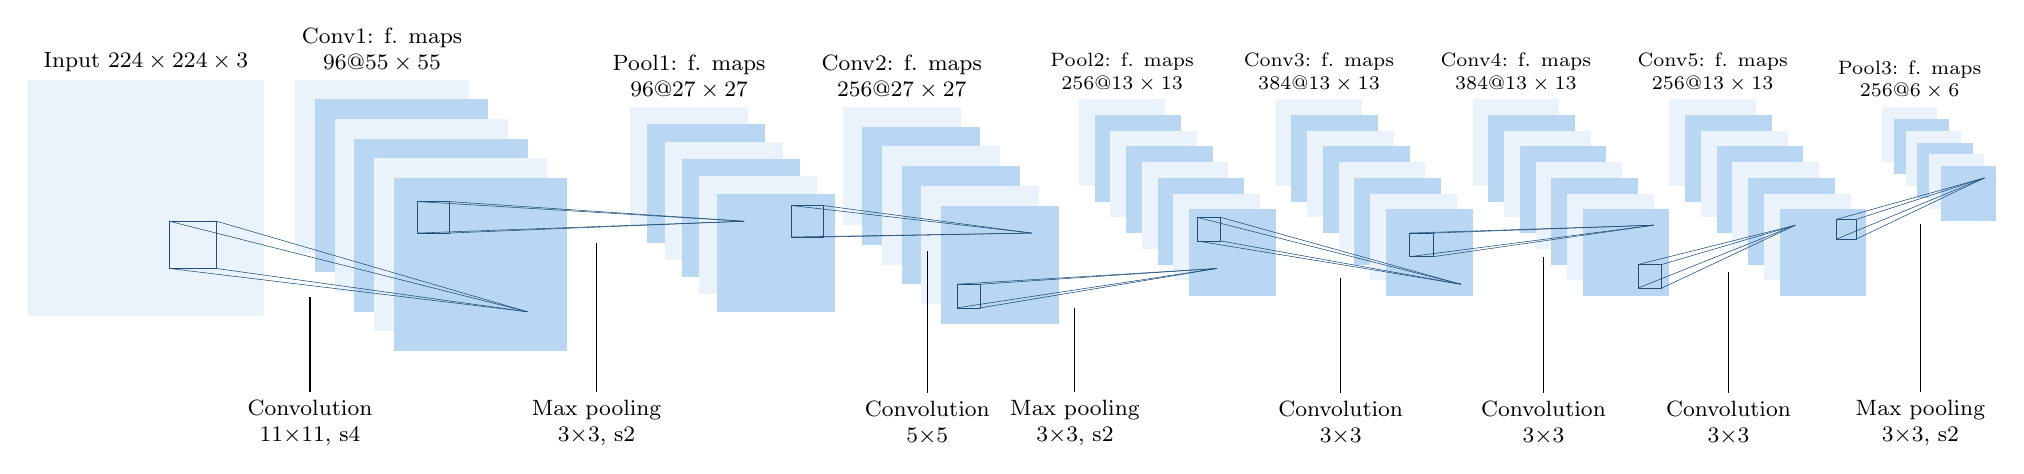
\begin{tikzpicture}[
    font=\footnotesize, line join=round,
    every node/.style={outer sep=0pt, inner sep=0pt, align=center},
    s/.style={minimum size=#1},
    ed/.style={shorten <=#1}
  ]

  % ========== 特征图堆宏 ==========
  \newcommand{\stack}[4]{%
    \foreach \i in {0,...,#2} {%
      \ifodd\i
        \node[s=#3, fill=fillB] (#1\i) at (#4*\i,-#4*\i) {};
      \else
        \node[s=#3, fill=fillA] (#1\i) at (#4*\i,-#4*\i) {};
      \fi
    }%
  }

  % ========== 输入 ==========
  \node[s=3cm, fill=fillA] (in0) at (0,0.8) {};

  % ========== 特征图堆 ==========
  \begin{scope}[xshift=3.0cm, yshift=1.2cm]  \stack{a}{5}{2.2cm}{.25} \end{scope}  % Conv1 96@55
  \begin{scope}[xshift=6.9cm, yshift=1.2cm]  \stack{b}{5}{1.5cm}{.22} \end{scope}  % Pool1 96@27
  \begin{scope}[xshift=9.6cm, yshift=1.2cm]  \stack{c}{5}{1.5cm}{.25} \end{scope}  % Conv2 256@27
  \begin{scope}[xshift=12.4cm, yshift=1.5cm] \stack{d}{7}{1.1cm}{.2}  \end{scope}  % Pool2 256@13
  \begin{scope}[xshift=14.9cm, yshift=1.5cm] \stack{e}{7}{1.1cm}{.2}  \end{scope}  % Conv3 384@13
  \begin{scope}[xshift=17.4cm, yshift=1.5cm] \stack{f}{7}{1.1cm}{.2}  \end{scope}  % Conv4 384@13
  \begin{scope}[xshift=19.9cm, yshift=1.5cm] \stack{g}{7}{1.1cm}{.2}  \end{scope}  % Conv5 256@13
  \begin{scope}[xshift=22.4cm, yshift=1.6cm] \stack{h}{5}{.7cm}{.15} \end{scope}   % Pool3 256@6

  % ========== 顶部层名标注 ==========
  \node[above=1mm] at (in0.north) {Input $224\times224\times3$};
  \node[above=1mm] at (a0.north) {Conv1: f. maps\\96@$55\times55$};
  \node[above=1mm] at (b0.north) {Pool1: f. maps\\96@$27\times27$};
  \node[above=1mm] at (c0.north) {Conv2: f. maps\\256@$27\times27$};
  \node[above=1mm, font=\scriptsize] at (d0.north) {Pool2: f. maps\\256@$13\times13$};
  \node[above=1mm, font=\scriptsize] at (e0.north) {Conv3: f. maps\\384@$13\times13$};
  \node[above=1mm, font=\scriptsize] at (f0.north) {Conv4: f. maps\\384@$13\times13$};
  \node[above=1mm, font=\scriptsize] at (g0.north) {Conv5: f. maps\\256@$13\times13$};
  \node[above=1mm, font=\scriptsize] at (h0.north) {Pool3: f. maps\\256@$6\times6$};

  % ========== 感受野小窗口 + 收敛线 ==========
  % Input -> Conv1
  \node[draw,linecol, very thin, s=.6cm] (win1) at ($(in0.center)+(.6,-.6)$) {};
  \foreach \i in {north west,north east,south west,south east}
    \draw[very thin,linecol] (win1.\i)--coordinate[pos=.3](w1) ($(a5.center)+(.6,-.6)$);
  % Conv1 -> Pool1
  \node[draw,linecol, very thin, s=.4cm] (win2) at ($(a5.center)+(-.6,.6)$) {};
  \foreach \i in {north west,north east,south west,south east}
    \draw[very thin,linecol] (win2.\i)--coordinate[pos=.5](w2) ($(b5.center)+(-.4,.4)$);
  % Pool1 -> Conv2
  \node[draw,linecol, very thin, s=.4cm] (win3) at ($(b5.center)+(.4,.4)$) {};
  \foreach \i in {north west,north east,south west,south east}
    \draw[very thin,linecol] (win3.\i)--coordinate[pos=.5](w3) ($(c5.center)+(.4,.4)$);
  % Conv2 -> Pool2
  \node[draw,linecol, very thin, s=.3cm] (win4) at ($(c5.center)+(-.4,-.4)$) {};
  \foreach \i in {north west,north east,south west,south east}
    \draw[very thin,linecol] (win4.\i)--coordinate[pos=.4](w4) ($(d7.center)+(-.2,-.2)$);
  % Pool2 -> Conv3（窗口改到源堆左上，收敛点在目标堆左上）
  \node[draw,linecol, very thin, s=.3cm] (win5) at ($(d7.center)+(-.3,.3)$) {};
  \foreach \i in {north west,north east,south west,south east}
    \draw[very thin,linecol] (win5.\i)--coordinate[pos=.5](w5) ($(e7.center)+(.4,-.4)$);
  % Conv3 -> Conv4（同样处理）
  \node[draw,linecol, very thin, s=.3cm] (win6) at ($(e7.center)+(-.1,.1)$) {};
  \foreach \i in {north west,north east,south west,south east}
    \draw[very thin,linecol] (win6.\i)--coordinate[pos=.5](w6) ($(f7.center)+(.35,.35)$);
  % Conv4 -> Conv5（同样处理）
  \node[draw,linecol, very thin, s=.3cm] (win7) at ($(f7.center)+(.3,-.3)$) {};
  \foreach \i in {north west,north east,south west,south east}
    \draw[very thin,linecol] (win7.\i)--coordinate[pos=.5](w7) ($(g7.center)+(-.35,.35)$);
  % Conv5 -> Pool3
  \node[draw,linecol, very thin, s=.25cm] (win8) at ($(g7.center)+(.3,.3)$) {};
  \foreach \i in {north west,north east,south west,south east}
    \draw[very thin,linecol] (win8.\i)--coordinate[pos=.5](w8) ($(h5.center)+(.2,.2)$);

  % ========== 底部操作说明（一行对齐）==========
  \node (L1) at ($(w1)+(0,-1.8)$) {Convolution\\11$\times$11, s4};
  \draw[ed=2mm] (w1)--([yshift=1mm]L1.north);
  \node (L2) at (w2|-L1) {Max pooling\\3$\times$3, s2};
  \draw[ed=2mm] (w2)--([yshift=1mm]L2.north);
  \node (L3) at (w3|-L1) {Convolution\\5$\times$5};
  \draw[ed=2mm] (w3)--([yshift=1mm]L3.north);
  \node (L4) at (w4|-L1) {Max pooling\\3$\times$3, s2};
  \draw[ed=2mm] (w4)--([yshift=1mm]L4.north);
  \node (L5) at (w5|-L1) {Convolution\\3$\times$3};
  \draw[ed=2mm] (w5)--([yshift=1mm]L5.north);
  \node (L6) at (w6|-L1) {Convolution\\3$\times$3};
  \draw[ed=2mm] (w6)--([yshift=1mm]L6.north);
  \node (L7) at (w7|-L1) {Convolution\\3$\times$3};
  \draw[ed=2mm] (w7)--([yshift=1mm]L7.north);
  \node (L8) at (w8|-L1) {Max pooling\\3$\times$3, s2};
  \draw[ed=2mm] (w8)--([yshift=1mm]L8.north);

\end{tikzpicture}
\end{document}